%%%%%%%%%%%%%%%%%%%%%%%%%%%%%%%%%%%%%%%%%
% Short Sectioned Assignment
% LaTeX Template
% Version 1.0 (5/5/12)
%
% This template has been downloaded from:
% http://www.LaTeXTemplates.com
%
% Original author:
% Frits Wenneker (http://www.howtotex.com)
%
% License:
% CC BY-NC-SA 3.0 (http://creativecommons.org/licenses/by-nc-sa/3.0/)
%
%%%%%%%%%%%%%%%%%%%%%%%%%%%%%%%%%%%%%%%%%

%----------------------------------------------------------------------------------------
%	PACKAGES AND OTHER DOCUMENT CONFIGURATIONS
%----------------------------------------------------------------------------------------

\documentclass[paper=a4, fontsize=11pt]{scrartcl} % A4 paper and 11pt font size

\usepackage[T1]{fontenc} % Use 8-bit encoding that has 256 glyphs
\usepackage{fourier} % Use the Adobe Utopia font for the document - comment this line to return to the LaTeX default
\usepackage[english]{babel} % English language/hyphenation
\usepackage{amsmath,amsfonts,amsthm} % Math packages

\usepackage{lipsum} % Used for inserting dummy 'Lorem ipsum' text into the template

\usepackage{sectsty} % Allows customizing section commands

\usepackage{graphicx}
\usepackage{todonotes}

\allsectionsfont{\centering \normalfont\scshape} % Make all sections centered, the default font and small caps

\usepackage{fancyhdr} % Custom headers and footers
\pagestyle{fancyplain} % Makes all pages in the document conform to the custom headers and footers
\fancyhead{} % No page header - if you want one, create it in the same way as the footers below
\fancyfoot[L]{} % Empty left footer
\fancyfoot[C]{} % Empty center footer
\fancyfoot[R]{\thepage} % Page numbering for right footer
\renewcommand{\headrulewidth}{0pt} % Remove header underlines
\renewcommand{\footrulewidth}{0pt} % Remove footer underlines
\setlength{\headheight}{13.6pt} % Customize the height of the header

\numberwithin{equation}{section} % Number equations within sections (i.e. 1.1, 1.2, 2.1, 2.2 instead of 1, 2, 3, 4)
\numberwithin{figure}{section} % Number figures within sections (i.e. 1.1, 1.2, 2.1, 2.2 instead of 1, 2, 3, 4)
\numberwithin{table}{section} % Number tables within sections (i.e. 1.1, 1.2, 2.1, 2.2 instead of 1, 2, 3, 4)

\setlength\parindent{0pt} % Removes all indentation from paragraphs - comment this line for an assignment with lots of text

%----------------------------------------------------------------------------------------
%	TITLE SECTION
%----------------------------------------------------------------------------------------

\newcommand{\horrule}[1]{\rule{\linewidth}{#1}} % Create horizontal rule command with 1 argument of height

\title{	
\normalfont \normalsize 
\textsc{university, school or department name} \\ [25pt] % Your university, school and/or department name(s)
\horrule{0.5pt} \\[0.4cm] % Thin top horizontal rule
\huge Assignment Title \\ % The assignment title
\horrule{2pt} \\[0.5cm] % Thick bottom horizontal rule
}

\author{John Smith} % Your name

\date{\normalsize\today} % Today's date or a custom date

\begin{document}

\maketitle % Print the title

%----------------------------------------------------------------------------------------
%	PROBLEM 1
%----------------------------------------------------------------------------------------

\section{Our Task}

You should pick a number of 2D (or optionally 3D) datasets (where the variables correspond to the coordinates in the 2D or 3D space), and demonstrate how different settings of the parameter k in k-NN modify the decision boundary. Your solution should work with arbitrary number of classes.
Provide an interface that visualises the data set and its classes. In that interface, provide controls where the user can select a k value, and colour the points in the space according to which class they would get classified into. A simple approach is to iterate over all your points in the visualisation grid and ask the classifier for the classification of each point.

Finally, provide an option to the user to select a training/test set split, and indicate the classification of the test set in your plot.
The data sets you provide should contain examples where low numbers of k are superior, as well as examples where higher number of k are more accurate.

\section{Implementation}

We used R as a wrapper for Weka and plotted the result with the native functionality in R.

\section{Evaluation}
Our Data Set were 
\begin{enumerate}
\item
The 'Skin-NonSkin' Data Set, which is a collection of RGB-values and the 4th attribute states whether this is a skin color or not
\item
A truncation of the iris data set, with a removed column to fit the data to 3 dimensions
\item
\todo[inline]{... a third data set}
\end{enumerate}

The knn nearest neighbor performs especially well if we have a balanced data set with separated spaces where one of the class values is dominating. Figure \ref{fig:skin:predicted:k5} shows the prediction of K-Nearest-Neighbor for the 'Skin-Nonskin' data set. Obviously, there are a certain space where all the actual skin colors are located. This is an important fact, which facilitates the prediction of instances. In figure \ref{fig:skin:correct:k5} one can see the same data set visualized based on the correctness of the prediction. Black marks belong to correct instances and white marks belong to misclassified instances. In this example, k-nn performs very well, only few instances lying on the border to the skin color space are misclassified.

\begin{figure}[\textwidth]
    \begin{center}
        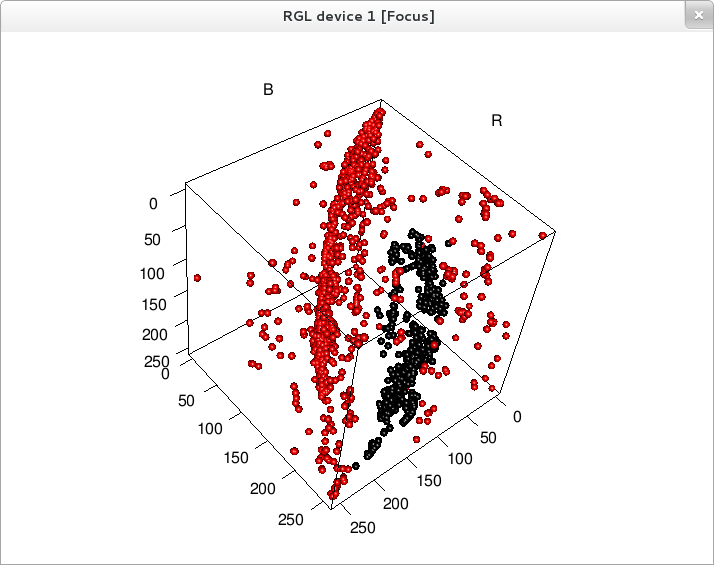
\includegraphics[width=\textwidth]{Skin_predicted_k5}
    \end{center}
    \caption['Skin-NonSkin' prediction with k=5]{The 'Skin-NonSkin' Data Set, colored by the predicted class attribute, with 5 neighbors as K parameter.}
    \label{fig:skin:predicted:k5}
\end{figure}

\begin{figure}[\textwidth]
    \begin{center}
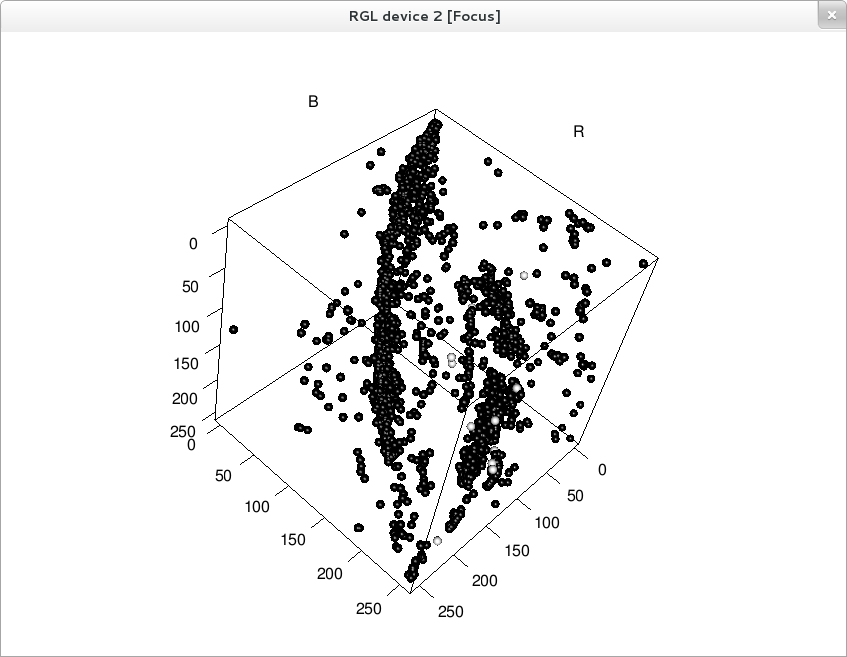
\includegraphics[width=\textwidth]{Skin_correct_k5}
    \end{center}
\caption['Skin-NonSkin' correctness with k=5]{The 'Skin-NonSkin' Data Set, colored by correct or misclassified instance, with 5 neighbors as K parameter.}
\label{fig:skin:correct:k5}
\end{figure}

\begin{figure}[\textwidth]
    \begin{center}
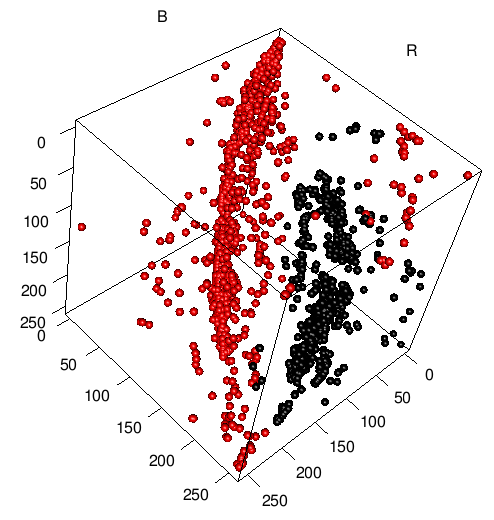
\includegraphics[width=\textwidth]{Skin_predicted_k100}
    \end{center}
\caption['Skin-NonSkin' prediction with k=100]{The 'Skin-NonSkin' Data Set, colored by the predicted class attribute, with 100 neighbors as K parameter.}
\label{fig:skin:predicted:k100}
\end{figure}


If we raise the K-paramter up to 100, we get worse results. As seen in figure \ref{fig:skin:predicted:k100} the K-NN algorithm misclassfies more instances that are located in one corner of the RGB space. Hence, we can see more white marks in figure \ref{fig:skin:correct:k100}.

\begin{figure}[\textwidth]
    \begin{center}
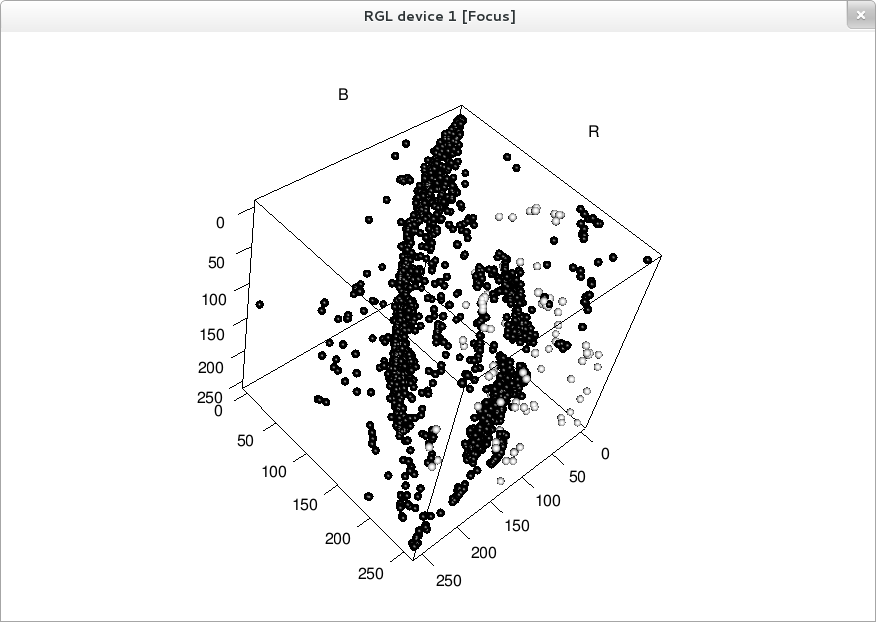
\includegraphics[width=\textwidth]{Skin_correct_k100}
    \end{center}
\caption['Skin-NonSkin' correctness with k=100]{The 'Skin-NonSkin' Data Set, colored by correct or misclassified instance, with 100 neighbors as K parameter.}
\label{fig:skin:correct:k100}
\end{figure}

\subsection{Data Sets}
\todo[inline]{Wich data sets did we used?}
\end{document}
